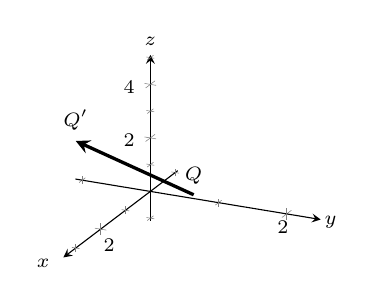
\begin{tikzpicture}
\begin{axis}%
[width=175pt,tick label style={font=\scriptsize},axis on top,
			axis lines=center,
			%y dir=reverse,
			name=myplot,
			view={115}{30},
			minor x tick num=1,
			minor y tick num=1,
			minor z tick num=1,
			%extra y ticks={-5,-3,...,7},%
			ymin=-1.1,ymax=2.5,%
			xmin=-1.1,xmax=3.5,
			zmin=-1.1, zmax=5.1%
]

\draw [->,>=stealth,very thick] (axis cs:1,1,1) node [above] {\scriptsize $Q$} -- (axis cs:3,0,4)node [above] {\scriptsize $Q'$};

\threedlines[{\colortwo}]{3}{0}{4}
\threedlines[{\colortwo}]{1}{1}{1}



\end{axis}


\node [right] at (myplot.right of origin)[shift={(-12pt,-11pt)}] {\scriptsize $y$};
\node [right] at (myplot.right of origin)[shift={(-116pt,-26pt)}] {\scriptsize $x$};
\node [above] at (myplot.above origin) [shift={(0,-12pt)}] {\scriptsize $z$};
\end{tikzpicture}








